%% 
%% Copyright 2007-2019 Elsevier Ltd
%% 
%% This file is part of the 'Elsarticle Bundle'.
%% ---------------------------------------------
%% 
%% It may be distributed under the conditions of the LaTeX Project Public
%% License, either version 1.2 of this license or (at your option) any
%% later version.  The latest version of this license is in
%%    http://www.latex-project.org/lppl.txt
%% and version 1.2 or later is part of all distributions of LaTeX
%% version 1999/12/01 or later.
%% 
%% The list of all files belonging to the 'Elsarticle Bundle' is
%% given in the file `manifest.txt'.
%% 
%% Template article for Elsevier's document class `elsarticle'
%% with harvard style bibliographic references

\documentclass[preprint,12pt,authoryear]{elsarticle}

%% Use the option review to obtain double line spacing
%% \documentclass[authoryear,preprint,review,12pt]{elsarticle}

%% Use the options 1p,twocolumn; 3p; 3p,twocolumn; 5p; or 5p,twocolumn
%% for a journal layout:
%% \documentclass[final,1p,times,authoryear]{elsarticle}
%% \documentclass[final,1p,times,twocolumn,authoryear]{elsarticle}
%% \documentclass[final,3p,times,authoryear]{elsarticle}
%% \documentclass[final,3p,times,twocolumn,authoryear]{elsarticle}
%% \documentclass[final,5p,times,authoryear]{elsarticle}
%% \documentclass[final,5p,times,twocolumn,authoryear]{elsarticle}

%% For including figures, graphicx.sty has been loaded in
%% elsarticle.cls. If you prefer to use the old commands
%% please give \usepackage{epsfig}

%% The amssymb package provides various useful mathematical symbols
\usepackage{amssymb}
%% The amsthm package provides extended theorem environments
%% \usepackage{amsthm}

%% The lineno packages adds line numbers. Start line numbering with
%% \begin{linenumbers}, end it with \end{linenumbers}. Or switch it on
%% for the whole article with \linenumbers.
%% \usepackage{lineno}

\usepackage[utf8x]{inputenc}
\usepackage{longtable}
\usepackage{pdflscape}
\usepackage{multirow}

\bibliographystyle{elsarticle-harv}%\biboptions{authoryear}

\journal{Applied Soft Computing}

\begin{document}

\begin{frontmatter}

%% Title, authors and addresses

%% use the tnoteref command within \title for footnotes;
%% use the tnotetext command for theassociated footnote;
%% use the fnref command within \author or \address for footnotes;
%% use the fntext command for theassociated footnote;
%% use the corref command within \author for corresponding author footnotes;
%% use the cortext command for theassociated footnote;
%% use the ead command for the email address,
%% and the form \ead[url] for the home page:

\title{TITULO: Lorem ipsum dolor sit amet, consectetur adipiscing elit. Vestibulum tristique.}

\author[1]{Felipe Andr\'e Zeiser}
\ead{felipezeiser@ifsul.edu.br}

\address[1]{Instituto Federal Sul-Rio-Grandense - Campus de Sapucaia do Sul}


\begin{abstract}
Lorem ipsum dolor sit amet, consectetur adipiscing elit. Fusce euismod hendrerit lacus, nec auctor tortor consectetur sed. Fusce vehicula metus ac sem elementum sodales. Etiam sollicitudin sem at dui efficitur lobortis. Morbi suscipit urna ut elit interdum, vel cursus metus varius. Duis in hendrerit est. Vivamus finibus porta risus sit amet venenatis. Nunc iaculis sodales quam maximus tincidunt. Cras in fringilla ligula. Fusce condimentum ligula at neque porta, quis lobortis sem auctor. Mauris eu neque quis libero convallis volutpat ut luctus mauris. Vivamus eu metus tellus. Etiam quis enim nulla. Suspendisse potenti. Duis vel convallis mi, sit amet pulvinar elit. Aliquam bibendum nisl vel lectus gravida iaculis.

\end{abstract}

\begin{keyword}
Lorem; ipsum; dolor; sit; amet;
\end{keyword}

\end{frontmatter}

%% main text
\section{Introduction}

Lorem ipsum dolor sit amet, consectetur adipiscing elit. Cras congue hendrerit ligula, nec rhoncus velit. Aenean posuere justo ut lectus tristique, et tincidunt enim consectetur. Morbi ac massa nec arcu egestas lobortis eget nec augue. Sed suscipit est nec auctor tempus. Curabitur dapibus nisi non nisl maximus fringilla. Maecenas non metus sed nunc faucibus ullamcorper. Maecenas dapibus aliquam urna quis sagittis. Lorem ipsum dolor sit amet, consectetur adipiscing elit.

% Segundo Montenegro et al. (2019), a revisão sistemática permite uma reprodutibilidade do estudo.

% A revisão sistemática permite uma reprodutibilidade do estudo (MONTENEGRO et al., 2019)


Segundo \cite{MONTENEGRO2019}, a revisão sistemática permite uma reprodutibilidade do estudo.

A revisão sistemática permite uma reprodutibilidade do estudo \citep{MONTENEGRO2019}. 

\cite{YASSIN2018}

\begin{table}[!htpb]
    \centering
    \begin{tabular}{|c|c|c|c|}
         \hline
         \textbf{Dado 1} & \textbf{Dado 2} & \textbf{Dado 3} & \textbf{Dado 4}  \\
         \hline
         \multicolumn{2}{|c|}{Gastos} & teste & teste\\
         \hline
         Dado Inicial & \multicolumn{3}{|c|}{Gastos} \\
         \hline
         \multicolumn{4}{|c|}{Gastos} \\
         \hline
    \end{tabular}
    \caption{Minha legenda para uma tabela com colunas e linhas 'mescladas'.}
    \label{tab:my_label}
\end{table}

\begin{table}[!htpb]
    \centering
    \begin{tabular}{|p{7cm}|c|c|c|c|}
    \hline
         \textbf{Dado 1} & \textbf{Dado 2}  & \textbf{Dado 3} & \textbf{Dado 4} & \textbf{Dado 5}\\         
         \hline
         \multirow{2}{*}{duas linha} & Teste  & Teste & Teste & Teste \\
         \cline{2-2} \cline{4-4}
         & Teste & Teste & Teste & Teste\\
         \hline
         \multirow{4}{*}{\rotatebox[origin=c]{90}{tres linhas}} & Teste  & Teste & Teste & Teste \\
         \cline{2-5}
         & linha 4& & &\\
         \cline{2-5}
         & linha 5& & &\\
         \cline{2-5}
         & linha 5& & &\\
         \hline
    \end{tabular}
    \caption{Caption}
    \label{tab:my_label}
\end{table}

\begin{longtable}{p{6.5cm}p{3.5cm}p{0.3cm}p{0.5cm}}
    \caption{Tabela Gigante}
    \label{tab:gigante}\\
    
    \hline
    \multicolumn{1}{c}{\textbf{Referencia}} & \multicolumn{1}{c}{\textbf{Editora}} & \multicolumn{1}{c}{\textbf{h5}} & \multicolumn{1}{c}{\textbf{SJR}} \\
    \hline
    \endfirsthead
    
    \hline \multicolumn{4}{r}{{Continua na próxima página}} \\ \hline
    \multicolumn{2}{c}{MAIS UMA LINHA}&\multicolumn{2}{c}{MAIS UMA INFO}\\
    \hline
        \endfoot
    
    \multicolumn{4}{c}{{\bfseries \tablename\ \thetable{} -- continuação da página anterior}} \\
        \hline 
        \multicolumn{1}{c}{\textbf{Referencia}}&\multicolumn{1}{c}{\textbf{Editora}}&\multicolumn{1}{c}{\textbf{h5}}&\multicolumn{1}{c}{\textbf{SJR}}\\
        \hline
        \endhead
        
        
        \multicolumn{4}{r}{FIM DA TABELA}\\
        \hline \hline
        \endlastfoot
        
        \citet{GUO2019}               & Nature                  & 151 & 1,414 \\
            \citet{VO2019}                & Elsevier                & 94  & 1,62  \\
            \citet{XIE2019}               & Frontiers               & 59  & 1,888 \\
            \citet{LI2019}                & IEEE                    & 57  & 0,609 \\
            \citet{MURTAZA2019}           & Springer                & 45  & 0,335 \\
            \citet{DAS2019}               & Elsevier                & 39  & 0,57  \\
            \citet{MITTAL2019}            & Elsevier                & 32  & 1,278 \\
            \citet{ALOM2019}              & Springer                & 29  & 0,666 \\
            \citet{ROY2019}               & Elsevier                & 29  & 0,805 \\
            \citet{GHAZVINIANZANJANI2019} & SPIE                    & 16  & 0,6   \\
            \citet{SABEENABEEVI2019}      & Elsevier                & 16  & 0,438 \\
            \citet{ALQUDAH2019}           & Taylor \& Francis       & 15  & 0,207 \\
            \citet{CRUZROA2018}           & PLOS                    & 180 & 1,1   \\
            \citet{OLIVEIRA2018}          & Elsevier                & 92  & 1,19  \\
            \citet{GECER2018}             & Elsevier                & 74  & 1,363 \\
            \citet{ZHENG2018}             & IEEE                    & 66  & 2,188 \\
            \citet{LI2018}                & Elsevier                & 57  & 2,452 \\
            \citet{BARDOU2018}            & IEEE                    & 57  & 0,609 \\
            \citet{FONDON2018}            & Elsevier                & 39  & 0,57  \\
            \citet{GANDOMKAR2018a}        & Elsevier                & 32  & 1,025 \\
            \citet{SAHA2018a}             & Elsevier                & 29  & 0,805 \\
            \citet{FENG2018}              & Springer                & 28  & 0,625 \\
            \citet{PAN2018}               & Elsevier                & 27  & 0,402 \\
            \citet{HAN2017}               & Nature                  & 151 & 1,414 \\
            \citet{ZHENG2017}             & Elsevier                & 74  & 1,363 \\
            \citet{WAN2017a}              & Elsevier                & 71  & 0,996 \\
            \citet{PAN2017}               & Elsevier                & 71  & 0,996 \\
            \citet{WAN2017b}              & Elsevier                & 71  & 0,996 \\
            \citet{WAHAB2017}             & Elsevier                & 39  & 0,57  \\
            \citet{BEJNORDI2017}          & SPIE                    & 16  & 0,6   \\
            \citet{KRAWCZYK2016}          & Elsevier                & 77  & 1,216 \\
            \citet{XU2016}                & IEEE                    & 66  & 2,188 \\
            \citet{ZHANG2016}             & IEEE                    & 56  & 1,122 \\
            \citet{CHAN2016}              & The Royal Soc.          & 32  & 1,131 \\
            \citet{BALAZSI2016}           & SPIE                    & 16  & 0,6   \\
            \citet{KORKMAZ2016}           & Springer                & 11  & 0,61  \\
            \citet{TASHK2015}             & Elsevier                & 67  & 0,873 \\
            \citet{ZHANG2015}             & IEEE                    & 66  & 2,188 \\
            \citet{KHAN2015}              & IEEE                    & 56  & 1,122 \\
            \citet{WANG2014}              & SPIE                    & 16  & 0,6   \\
            \citet{LOUKAS2013}            & Hindawi                 & 31  & 0,414 \\
            \citet{ISSACNIWAS2012}        & Springer                & 45  & 0,565 \\
            \citet{DUNDAR2011}            & IEEE                    & 69  & 1,256\\
            \citet{DUNDAR2011}            & IEEE                    & 69  & 1,256\\
            \citet{DUNDAR2011}            & IEEE                    & 69  & 1,256\\
            \citet{DUNDAR2011}            & IEEE                    & 69  & 1,256\\
            \citet{DUNDAR2011}            & IEEE                    & 69  & 1,256\\
            \citet{DUNDAR2011}            & IEEE                    & 69  & 1,256\\
            \citet{DUNDAR2011}            & IEEE                    & 69  & 1,256\\
            \citet{DUNDAR2011}            & IEEE                    & 69  & 1,256\\
            \citet{DUNDAR2011}            & IEEE                    & 69  & 1,256\\
            \citet{DUNDAR2011}            & IEEE                    & 69  & 1,256\\
            \citet{DUNDAR2011}            & IEEE                    & 69  & 1,256\\
            \citet{DUNDAR2011}            & IEEE                    & 69  & 1,256\\
            \citet{DUNDAR2011}            & IEEE                    & 69  & 1,256\\
            \citet{DUNDAR2011}            & IEEE                    & 69  & 1,256
\end{longtable}


\begin{figure}[htpb]
    \centering
    \begin{tabular}{cccc}
        \multirow{2}{*}{\rotatebox[origin=c]{90}{\textbf{rota rota rota rota}}} & & &\\
         &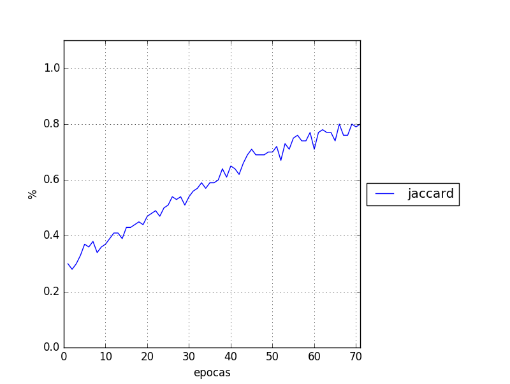
\includegraphics[scale=0.6]{images/jaccardmodeloA.png}& 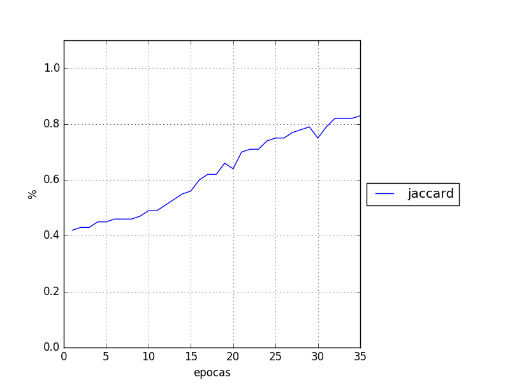
\includegraphics[scale=0.6]{images/jaccardmodeloB.png} & 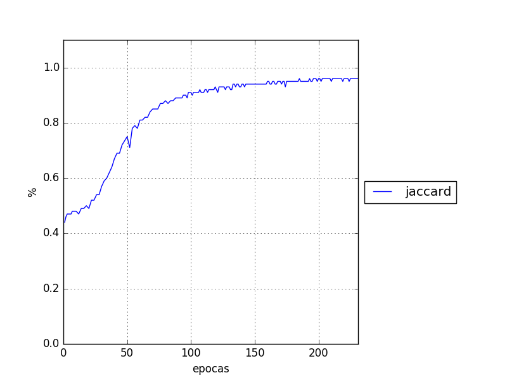
\includegraphics[scale=0.6]{images/jaccardmodeloC.png} \\
        &\textbf{(A)} & \textbf{(B)} & \textbf{(C)}
    \end{tabular}
    \caption{Figuras lado a lado}
    \label{fig:my_label}
\end{figure}

% \bibliographystyle{elsarticle-harv}
\bibliography{references}

\end{document}

\endinput
%%
%% End of file `elsarticle-template-harv.tex'.
